\documentclass[12pt, a4paper]{article}

\usepackage[english]{babel}
\usepackage[utf8]{inputenc}
\usepackage{amsmath}
\usepackage{graphicx}
\usepackage{csquotes}
\usepackage{amssymb}


\title{\textbf{Genomic Computing Evaluation}\\Assignment 3: NGS Data Processing}
\author{Fabrizio Frasca}
\date{\today}

\begin{document}
	
	\maketitle
	\clearpage
	
	\section*{Introduction}
	
	\begin{verbatim}
	mkdir homework
	cd homework
	ln -sn /home/lriva/lesson/homeworkFastqfiles/gata1.fastq .
	ln -sn /home/lriva/lesson/homeworkFastqfiles/tal1.fastq .
	ln -sn /home/lriva/lesson/homeworkFastqfiles/input.fastq .
	ln -sn /home/lriva/public_html/lesson/chromsizes.tab .
	\end{verbatim}
	
	These three fastq files contain the results of 2 ChIP-seq experiments and 1 control experiment.
	GATA1 and TAL1 are two mouse transcription factors, please check out the details for these samples here:\\
	
	• http://www.ncbi.nlm.nih.gov/geo/query/acc.cgi?acc=GSM923575
	
	• http://www.ncbi.nlm.nih.gov/geo/query/acc.cgi?acc=GSM923582
	
	• http://www.ncbi.nlm.nih.gov/geo/query/acc.cgi?acc=GSM923585\\
	
	
	The .sra raw data were downloaded and they were converted in fatstq files using the fastq-dump utility. We took 10 million reads out of those files, corresponding to 40 million lines of the fastq files
	
	\section{Checking the quality of the raw data}
	
	\subsection{}
	
	\textbf{Use the /home/lriva/FastQC/fastqc tool to get a report for the quality for these three fastq files; write here below the commands that you would use for this purpose}
	
	It is sufficient to run fastqc with the .fastq files as input.
	
	\begin{verbatim}
	/home/lriva/FastQC/fastqc gata1.fastq
	/home/lriva/FastQC/fastqc tal1.fastq
	/home/lriva/FastQC/fastqc input.fastq
	\end{verbatim}
	
	\subsection{}
	\textbf{What is the length of the reads? Inspect the fastq files and the fastqc report}
	
	All the reads have length \textbf{41}. This can be captured by inspecting the \textit{fastqc\_data.txt} files in \textit{gata1\_fastqc}, \textit{tal1\_fastqc} and \textit{input\_fastqc} generated folders.
	
	For all the three files we can read the following:
	
	\begin{verbatim}
	>>Sequence Length Distribution  pass
	#Length Count
	41      1.0E7
	>>END_MODULE
	\end{verbatim}
	meaning that the three starting fastq files have all the reads of length 41.
	
	The .html fastqc reports cannot be studied because of the problems encountered with the ftp protocol.
	
	\section{Filtering the raw data}
	
	\subsection{}
	\textbf{Use the fastx\_artifacts\_filter to remove artifacts}
	
	The commands are:
	
	\begin{verbatim}
	fastx_artifacts_filter -Q 33 -v -i gata1.fastq -o gata1_artifacts.fastq
	fastx_artifacts_filter -Q 33 -v -i tal1.fastq -o tal1_artifacts.fastq
	fastx_artifacts_filter -Q 33 -v -i input.fastq -o input_artifacts.fastq
	\end{verbatim}
	
	where we have specified options -Q 33 to refer to the Illumina quality score scale and -i, -o, to specify the input and output files.
	
	\subsection{}
	\textbf{Use fastq\_quality\_trimmer to trim based with quality lower than 20, requiring a min final length of 30nt}
	
	We can use the following commands:
	
	\begin{verbatim}
	fastq_quality_trimmer -Q 33 -v -t 20 -l 30
	-i gata1_artifacts.fastq -o gata1_artifacts_trim.fastq
	fastq_quality_trimmer -Q 33 -v -t 20 -l 30
	-i tal1_artifacts.fastq -o tal1_artifacts_trim.fastq
	fastq_quality_trimmer -Q 33 -v -t 20 -l 30
	-i input_artifacts.fastq -o input_artifacts_trim.fastq	
	\end{verbatim}
	
	where we used -t 20 to set the quality cutoff threshold to 20 and -l 30 to impose the minimum final length to 30 of the trimmed reads.
	
	\subsection{}
	\textbf{Use fastq\_quality\_filter to keep only those reads with al least 80\% of high quality bases (quality $>$ 20)}
	
	The commands are:
	
	\begin{verbatim}
	fastq_quality_filter -Q 33 -v -q 21 -p 80
	-i gata1_artifacts_trim.fastq -o gata1_artifacts_trim_quality.fastq
	fastq_quality_filter -Q 33 -v -q 21 -p 80
	-i tal1_artifacts_trim.fastq -o tal1_artifacts_trim_quality.fastq
	fastq_quality_filter -Q 33 -v -q 21 -p 80
	-i input_artifacts_trim.fastq -o input_artifacts_trim_quality.fastq
	\end{verbatim}
	
	where -p 80 is to enforce that at least 80\% of the bases must be high quality, and -q 21 filters out all the reads with quality smaller than 21. The choice to go for 21 instead of 20 was made because -q option takes integers values and the requirement was for a quality \textit{strictly} greater than 20.
	
	\section{Checking the quality of the filtered data}
	
	\subsection{}
	\textbf{Use the /home/lriva/FastQC/fastqc tool to get a report for the quality for the filtered fastq files}
	
	The commands are, again:
	
	\begin{verbatim}
	/home/lriva/FastQC/fastqc gata1_artifacts_trim_quality.fastq
	/home/lriva/FastQC/fastqc tal1_artifacts_trim_quality.fastq
	/home/lriva/FastQC/fastqc input_artifacts_trim_quality.fastq
	\end{verbatim}
	
	\subsection{}
	\textbf{Compare the results of 3.1) with 1.1) and briefly describe differences}
	
	By comparing the generated files \textit{fastqc\_data.txt} for all the couples:
	\begin{itemize}
		\item input \textit{vs} input\_artifacts\_trim\_quality
		\item gata1 \textit{vs} gata1\_artifacts\_trim\_quality
		\item tal1 \textit{vs} tal1\_artifacts\_trim\_quality
	\end{itemize}
	it is possible to notice that, in general, all the filtering operations together significantly enhanced the average quality of the reads.

	In particular, the quality on the 'tail' is generally higher and less dispersed around its mean value - smaller interquartile difference. This causes the average-quality trend to be more constant, and we can indeed notice there no more heavy drops like before.

	Finally, also consider the 10th percentile on the tail is now generally much higher and the count for N bases on the starting and ending positions is greatly reduced, and this is because such bases are cleaved off by the trimming operation, being very poor quality bases.
	
	\subsection{}
	\textbf{Which sample got the more reads discarded? how many reads still remain for this sample?}
	
	Since the initial number of reads was 10 millions for all the three samples, it is sufficient to look for the sample which has the minimum number of lines in the filtered fastq file:
	
	\begin{verbatim}
	$ wc -l gata1_artifacts_trim_quality.fastq 
	38151468 gata1_artifacts_trim_quality.fastq
	
	$ wc -l tal1_artifacts_trim_quality.fastq 
	38484388 tal1_artifacts_trim_quality.fastq
	
	$ wc -l input_artifacts_trim_quality.fastq 
	38185936 input_artifacts_trim_quality.fastq
	\end{verbatim}
	
	The sample with the more reads discarded is \textbf{gata1} and the the number of reads still remaining for that sample is $38,151,468 \div 4$, that is \textbf{9,537,867}.
	
	\section{Reads alignment}
	
	\subsection{}
	Align the reads to the mm9 mouse genome; for each of the tasks here below, write below the commands that you would use to perform the required task
	
	\subsubsection{}
	\textbf{Determine the .sai file containing the bwa index alignments using the "bwa align" command}
	
	\begin{verbatim}
	bwa aln -t4 -f gata1.sai /db/bwa/0.6.2/mm9/mm9
	gata1_artifacts_trim_quality.fastq
	bwa aln -t4 -f tal1.sai /db/bwa/0.6.2/mm9/mm9
	tal1_artifacts_trim_quality.fastq
	bwa aln -t4 -f input.sai /db/bwa/0.6.2/mm9/mm9
	input_artifacts_trim_quality.fastq
	\end{verbatim}
	
	\subsubsection{}
	\textbf{Convert these coordinates in genomic coordinates using the "bwa samse" command, export the results using "samtools view" and finally sort the aligned reads based on their genomic positions using "samtools sort"}
	
	It is convenient the three commands \verb samse , \verb samtools \ \verb view \ and \verb samtools \ \verb sort \ in a pipelined fashion: 
	
	\begin{verbatim}
	bwa samse /db/bwa/0.6.2/mm9/mm9 gata1.sai
	      gata1_artifacts_trim_quality.fastq |
	              samtools view -ut /db/bwa/0.6.2/mm9/mm9 - |
	              samtools sort - gata1
	bwa samse /db/bwa/0.6.2/mm9/mm9 tal1.sai
	      tal1_artifacts_trim_quality.fastq |
	              samtools view -ut /db/bwa/0.6.2/mm9/mm9 - |
	              samtools sort - tal1
	bwa samse /db/bwa/0.6.2/mm9/mm9 input.sai
	      input_artifacts_trim_quality.fastq |
	              samtools view -ut /db/bwa/0.6.2/mm9/mm9 - |
	              samtools sort - input
	\end{verbatim}
	
	\subsubsection{}
	\textbf{Create an index files for quick access to the .bam file using the "samtools index" command}
	
	It is sufficient to call the command \verb samtools \ \verb index \ by passing as input the three .bam files obtained in the step before:
	\begin{verbatim}
	samtools index gata1.bam
	samtools index tal1.bam
	samtools index input.bam
	\end{verbatim}
	
	\subsection{} 
	\textbf{What is the percentage of reads successfully aligned? use the "samtools view" command playing with the "-c" and "-F 4" options; answer for all three filtered fastq files, also writing the commands that you would use to perform the required task}
	
	The three commands below output the number of successfully mapped reads:
	
	\begin{verbatim}
	$ samtools view -F 4 -c gata1.bam
	8606362
	$ samtools view -F 4 -c tal1.bam
	9292370
	$ samtools view -F 4 -c input.bam
	9303996
	\end{verbatim}
	
	Then we can calculate the percentages of successfully mapped reads as follows:
	\\
	$gata1_\text{\%} = 100 \times \dfrac{mapped\ filtered\ reads}{overall\ filtered\ reads} = 100 \times \dfrac{8606362}{9537867} \approx 90.23$\\\\
	$tal1_\text{\%} = 100 \times \dfrac{mapped\ filtered\ reads}{overall\ filtered\ reads} = 100 \times \dfrac{9292370}{9621097} \approx 96.58$\\\\
	$input_\text{\%} = 100 \times \dfrac{mapped\ filtered\ reads}{overall\ filtered\ reads} = 100 \times \dfrac{9303996}{9546484} \approx  97.45$\\
	
	\section{Peak calling}
	
	\subsection{}
	\textbf{Use MACS to call ChIP-seq peaks; write here below the commands that you would use to perform the required task}
	
	In order to perform peak calling, macs14 is used with the two transcription factors obtained .bam files as treatment (\verb|-t| parameter), and with the input obtained .bam file as control for both (\verb|-c| parameter).
	
	Here below the two commands:
	
	\begin{verbatim}
	macs14 -t gata1.bam -c input.bam -n gata1 -m 10,30
	    -f BAM -p 1e-8 -g mm -s 41 --diag
	macs14 -t tal1.bam -c input.bam -n tal1 -m 10,30
	    -f BAM -p 1e-8 -g mm -s 41 --diag
	\end{verbatim}
	
	Among all the other parameters: \verb|-p| is used to set the Pvalue cutoff for peak detection at 1e-8, \verb|-g| is to indicate the genome length is the one of the mouse, \verb|-s| is used to set the tag size to 41 and \verb|--diag| is to ask macs to perform saturation analysis for peaks in several enrichment-ratio intervals.
	
	\subsection{}
	\textbf{How many positive and negative peaks were identified? (where negative peaks, in MACS terms, could be intended here as False Positives)}
	
	The number of peaks can be retrieved by counting the number of lines in the \textit{gata1\_peaks.bed} and \textit{tal1\_peaks.bed} generated files:
	
	\begin{verbatim}
	
	$ wc -l gata1_peaks.bed
	2603
	
	$ wc -l tal1_peaks.bed
	1553
	
	\end{verbatim}
	
	The number of negative peaks can instead be computed by \textbf{subtracting $1$} to the number of lines in the \textit{gata1\_negative\_peaks.xls} and the \textit{tal1\_negative\_peaks.xls} generated files. This is because the .xls files contain a one-line header.
	
	\begin{verbatim}
	
	$ wc -l gata1_negative_peaks.xls
	8
	
	$ wc -l tal1_negative_peaks.xls
	8
	
	\end{verbatim}
	
	That is: both tal1 and gata1 have 7 negative peaks identified.
	
	\subsection{}
	\textbf{What is the overall expected False Discovery Rate?}
	
	The False Discovery Rate is defined as the expected value of the proportion of false discoveries among the discoveries: $ FDR = \mathbb{E}[ V / R ]$ where $V$ is the number of false positives and $R$ is the number of discoveries.
	
	MACS uses to compute the $FDR$ for each peak and store such values at the ninth column of the "peaks.xls" generated file. In order to compute the $FDR$ value for each peak it does the following:
	
	\begin{itemize}
		\item fix the pvalue threshold as the peak pvalue
		\item call peaks according to the set pvalue
		\item obtain $x$ peaks
		\item swap treatment and control and perform peak calling with the same pvalue
		\item obtain $y$ peaks
		\item estimate the $FDR$ as $\dfrac{y}{x}$
	\end{itemize}
	
	In order to compute an \textit{overall} expected False Discovery Rate one choice can be to act accordingly, so that FDRs for gata1 and tal1 can be estimated, respectively, as:
	
	$FDR_\text{gata1} = \dfrac{\text{gata1 negative peaks}}{\text{gata1 peaks}} = \dfrac{7}{2603} \approx{0.0027}$
	
	
	$FDR_\text{tal1} = \dfrac{\text{tal1 negative peaks}}{\text{tal1 peaks}} = \dfrac{7}{1553} \approx{0.0045}$
	
	\subsection{}
	\textbf{Regarding the False Negatives, what are gata1 and tal1 saturation levels with 90\% of the reads at an enrichment level of 20-40 fold?}
	
	To answer this question we have to inspect the \textit{gata1\_diag.xls } and \textit{tal1\_diag.xls} generated files. The value at the second row and third column refers to the coverage by a sampling of 90\% for the peaks with an enrichment rate in the interval 20-40, so this is the value we are looking for. We have:\\
	
	\textbf{gata1}: 90.28
	
	\textbf{tal1}: 96.38
	
	
	\section{Identifying the binding events shared by the two transcription factors and those that are specific}
	
	\subsection{}
	\textbf{Use the "intersectBed" command to identify how many peaks are shared between gata1 and tal1, based on the output of 5.1); write here below the commands that you would use to perform the required task and report the number of found peaks}
	
	The commands we can use in order to do this are:
	
	\begin{verbatim}
	$ bedtools intersect -a gata1_peaks.bed 
	      -b tal1_peaks.bed -wa > int.bed
	$ wc -l int.bed
	1228
	\end{verbatim}
	
	The result is that we have 1228 peaks which are shared between the two treatments.
	
	\subsection{}
	\textbf{Check the documentation of the "intersectBed" command to identify how many peaks are specific for GATA1; write here below the commands that you would use to perform the required task and report the number of found peaks}
	
	The option \verb|-v| can be used to extract regions of the "\verb|A|" sample which do not overlap with any region of the "\verb|B|" sample. From the manual:
	\begin{displayquote}
		\begin{align*}
			\textbf{-v} \quad & \text{Only report those entries in A that have no overlap in B.}\\
			& \text{Restricted by -f and -r.}
		\end{align*}
	\end{displayquote}
	
	Thus, we can use the following commands:
	
	\begin{verbatim}
	$ bedtools intersect -a gata1_peaks.bed
	      -b tal1_peaks.bed -v > int_gata1.bed
	$ wc -l int_gata1.bed
	1377
	\end{verbatim}
	
	\section{Displaying the results in the genome browser}
	
	\subsection{}
	\textbf{Generate the bw files to be exported in the genome browser; for each of the subtask here below, write below the commands that you would use to perform the required task}
	
	\subsubsection{}
	\textbf{Convert the bam files in bed files using the "bamToBed" command}
	
	Let's first remove possible duplicates:
	
	\begin{verbatim}
	samtools rmdup -s gata1.bam gata1.nodup.bam
	samtools rmdup -s tal1.bam tal1.nodup.bam
	samtools rmdup -s input.bam input.nodup.bam
	\end{verbatim}
	
	Then we can call the command of interest:
	
	\begin{verbatim}
	bamToBed -i gata1.nodup.bam > gata1.bed
	bamToBed -i tal1.nodup.bam > tal1.bed
	bamToBed -i input.nodup.bam > input.bed
	\end{verbatim}
	
	\subsubsection{}
	\textbf{Create in silico extension of the peaks coordinates adding 160 bases to the right side in a strand specific manner, use the "slopBed" command}
	
	The commands are:
	
	\begin{verbatim}
	bedtools slop -i gata1.bed -g chromsizes.tab -s -l 0 -r 160
	  > gata1_slop.bed
	bedtools slop -i tal1.bed -g chromsizes.tab -s -l 0 -r 160
	  > tal1_slop.bed
	bedtools slop -i input.bed -g chromsizes.tab -s -l 0 -r 160
	  > input_slop.bed
	\end{verbatim}
	
	\subsubsection{}
	\textbf{Determine the count of reads for each base in the genome using the "genomeCoverageBed" command}
	
	In order to determine the count \textit{for each base}, we should use the \verb|-d| option:
	
	\begin{verbatim}
	genomeCoverageBed -i gata1_slop.bed -g chromsizes.tab -d
	  > gata1_perbase.wiggle
	genomeCoverageBed -i tal1_slop.bed -g chromsizes.tab -d
	  > tal1_perbase.wiggle
	genomeCoverageBed -i input_slop.bed -g chromsizes.tab -d
	  > input_perbase.wiggle
	\end{verbatim}
	
	However, if we want to upload the files on the UCSC genome browser, a more suitable option is to generate the output in bedgraph format, in this way:
	
	\begin{verbatim}
	genomeCoverageBed -i gata1_slop.bed -g chromsizes.tab -bg
	  > gata1.wiggle
	genomeCoverageBed -i tal1_slop.bed -g chromsizes.tab -bg
	  > tal1.wiggle
	genomeCoverageBed -i input_slop.bed -g chromsizes.tab -bg
	  > input.wiggle
	\end{verbatim}
	
	\subsubsection{}
	\textbf{Convert the .wg file in its binary bigwig version using the "wigToBigWig" command}
	
	It is sufficient to use the commands:
	
	\begin{verbatim}
	wigToBigWig gata1.wiggle chromsizes.tab gata1.bw
	wigToBigWig tal1.wiggle chromsizes.tab tal1.bw
	wigToBigWig input.wiggle chromsizes.tab input.bw
	\end{verbatim}
	
	\subsubsection{}
	\textbf{Go to http://genome.ucsc.edu/ and create three custom tracks with the three .bw files created in 7.1.4) and provide screen-shots of the uploaded tracks}
	
	The tracks were uploaded by following \verb|My data > Custom Tracks|, by selecting
	
	\begin{alignat*}{2}
	& \text{clade:} && \text{Mammal}\\
	& \text{genome:} && \text{Mouse}\\
	& \text{assembly:\quad} && \text{July 2007 (NCBI37/mm9)}\\
	\end{alignat*}
	and, finally, by providing the following lines to be submitted:
	
	
	\begin{verbatim}
	track type=bigWig name="gata1"
	      bigDataUrl=http://bioserver.iit.ieo.eu/~lriva/homeworkbw/gata1.bw
	
	track type=bigWig name="tal1"
	      bigDataUrl=http://bioserver.iit.ieo.eu/~lriva/homeworkbw/tal1.bw
	
	track type=bigWig name="input"
	      bigDataUrl=http://bioserver.iit.ieo.eu/~lriva/homeworkbw/input.bw
	\end{verbatim}	
	
	Here is a screenshot of the successfully updated tracks:
	
	\begin{figure}[h]
		\centering
		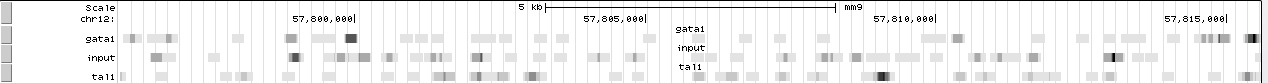
\includegraphics[width = 1.15\textwidth, height = .08\textheight]{browser_tracks}
		\caption{gata1, tal1 and input tracks uploaded on the UCSC genome browser}
		\label{fig:browser_tracks}
	\end{figure}
	
	\subsubsection{}
	\textbf{Based on 6.1) and 6.2) identify the genomic coordinates of one shared peak and of one peak specific for GATA1; browse to those locations and generate a plot in the genome browser reporting these two regions, and, finally, provide the screen-shot of the created plot}
	
	One shared peak is for the genomic coordinates \verb|chrX:53,981,724-53,982,059| and can be found in the \verb|int.bed| generated file. Figures \ref{fig:browser_int_dense} and \ref{fig:browser_int_full} depict the peaks in the UCSC genome browser.
	
	\begin{figure}[h]
		\centering
		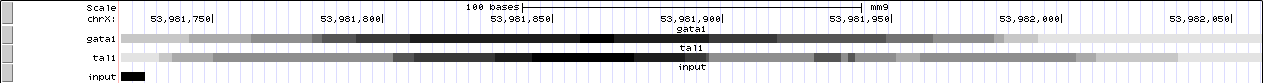
\includegraphics[width = 1.15\textwidth, height = .08\textheight]{browser_int_dense}
		\caption{shared peak for the coordinates: chrX:53,981,724-53,982,059, dense visualization}
		\label{fig:browser_int_dense}
	\end{figure}

	\begin{figure}[h]
		\centering
		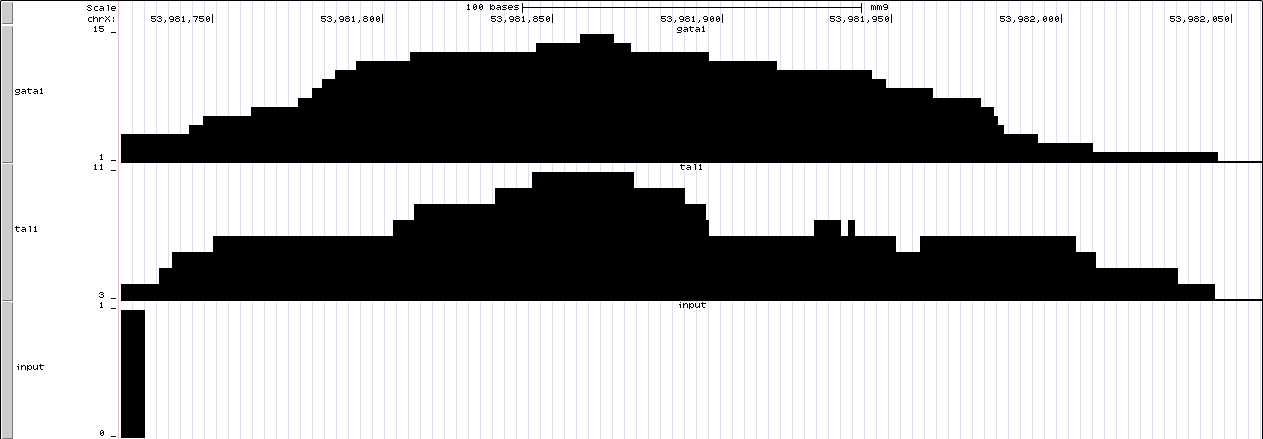
\includegraphics[width = 1.15\textwidth]{browser_int_full}
		\caption{shared peak for the coordinates: chrX:53,981,724-53,982,059, full visualization}
		\label{fig:browser_int_full}
	\end{figure}

	One peak specific for gata1 transcription factor is, instead, for the genomic coordinates \verb|chrX:131,741,773-131,742,135| and can be found in the \verb|int_gata1.bed| generated file. Figures \ref{fig:browser_spec_dense} and \ref{fig:browser_spec_full} depict the peak in the UCSC genome browser. 

	\begin{figure}[h]
		\centering
		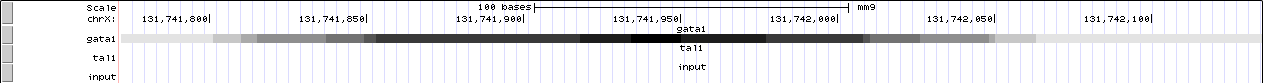
\includegraphics[width = 1.15\textwidth, height = .08\textheight]{browser_spec_dense}
		\caption{specific peak for the coordinates: chrX:131,741,773-131,742,135, dense visualization}
		\label{fig:browser_spec_dense}
	\end{figure}
	
	\clearpage
	
	\begin{figure}[t]
		\centering
		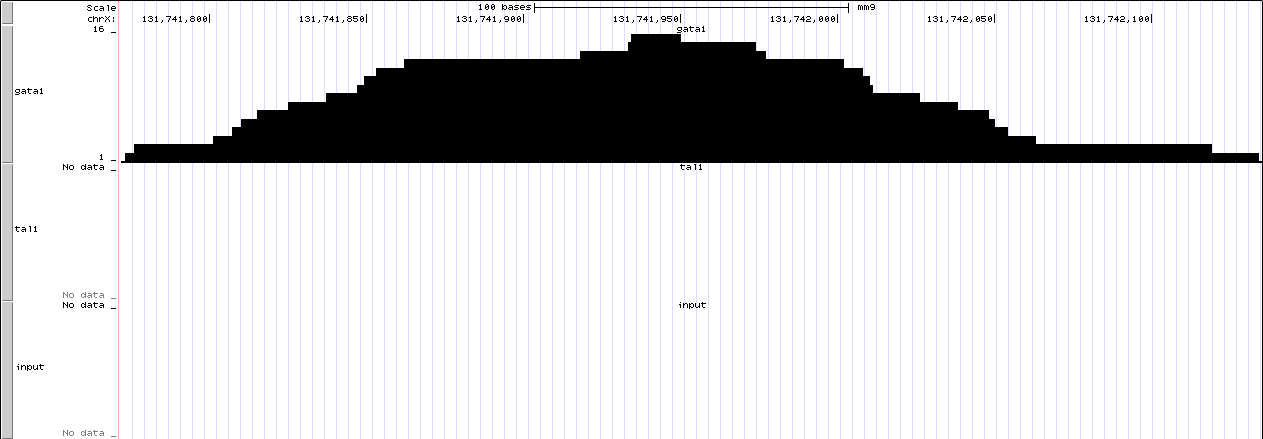
\includegraphics[width = 1.15\textwidth]{browser_spec_full}
		\caption{specific peak for the coordinates: chrX:131,741,773-131,742,135, full visualization}
		\label{fig:browser_spec_full}
	\end{figure}
	
	\section{Peaks annotation and motif finding with GREAT}
	
	\subsection{}
	\textbf{Use the "cut" linux command (with the -f argument) to generate the GREAT input files taking the first three columns of the .bed MACS peak files generated at 6.1) and 6.2)}
	
	In order to take the first three columns only, it is sufficient to use the \verb|-f 1-3| option with the cut command.
	
	\begin{verbatim}
	cut -f 1-3 int.bed > int_great.bed
	cut -f 1-3 spec_gata1.bed > spec_gata1_great.bed
	\end{verbatim}
	
	\subsection{}
	\textbf{Go to great.stanford.edu and upload the files obtained in 8.1) matching it to the mouse mm9 genome. Compare the motifs identified for the two peak sets; provide their screen shots and comment them briefly}
	
	As for the \textit{int\_great.bed} file, the reported results (figure \ref{fig:int_great}) correspond to the promoter motifs where a \textbf{joint} gata1 and tal1 binding is observed.
	
	As for the \textit{spec\_gata\_great.bed} file, the reported results (figure \ref{fig:spec_gata_great}) correspond to the promoter motifs where a \textbf{specific} gata1 binding is observed.
	
	The first motifs for both the two GREAT jobs have quite good pvalues.
	
	
	\clearpage
	
	\begin{figure}[h]
		\centering
		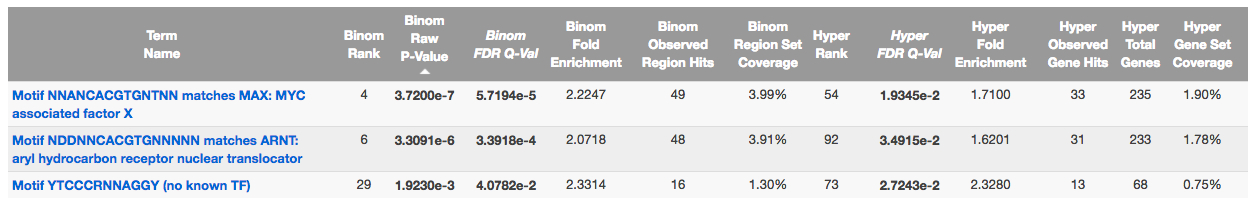
\includegraphics[width = .99\textwidth]{int_great}
		\caption{Predicted promoter motifs for the regions where both gata1 and tal1 transcription factors bind.}
		\label{fig:int_great}
	\end{figure}
	
	
	\begin{figure}[h]
		\centering
		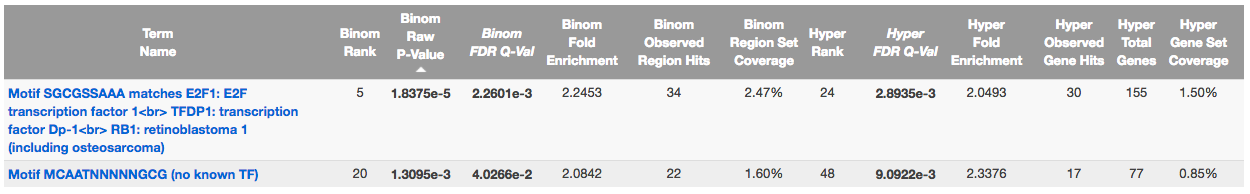
\includegraphics[width = .99\textwidth]{spec_gata_great}
		\caption{Predicted promoter motifs for the regions where only gata1 transcription factors binds.}
		\label{fig:spec_gata_great}
	\end{figure}
	
\end{document}